\documentclass[10pt,aspectratio=169]{beamer}

\usepackage[utf8]{inputenc}
\usepackage{amsmath}
\usepackage{amssymb}
\usepackage{amsfonts}
\usepackage{graphicx}
\usepackage{booktabs}
\usepackage{bm}

% Clean, modern slate-blue and cyan theme
\definecolor{primary}{RGB}{30, 41, 59} % Slate 800
\definecolor{secondary}{RGB}{71, 85, 105} % Slate 600
\definecolor{accent}{RGB}{14, 116, 144} % Cyan 700
\definecolor{background}{RGB}{248, 250, 252} % Slate 50

\usetheme{Madrid}
\usecolortheme{default}

\setbeamercolor{palette primary}{bg=primary, fg=white}
\setbeamercolor{palette secondary}{bg=secondary, fg=white}
\setbeamercolor{palette tertiary}{bg=accent, fg=white}
\setbeamercolor{palette quaternary}{bg=primary, fg=white}
\setbeamercolor{structure}{fg=accent}
\setbeamercolor{background canvas}{bg=background}

\setbeamertemplate{navigation symbols}{}

\graphicspath{{../../figures/publication/}}

\title[3D Quantum Percolation]{Physics and Numerics of 3D Quantum Percolation}
\subtitle{Transfer Matrix Method and Finite-Size Scaling}
\author[Tallosy \& Jaca]{Tallosy Peter, Jaca Gregorio}
\date[\today]{\today}

\begin{document}

% Slide 1: Title
\begin{frame}
  \titlepage
\end{frame}

% Slide 2: Table of Contents
\begin{frame}{Table of Contents}
  \tableofcontents
\end{frame}

\section{Introduction \& Foundations}

% Slide 3: Tight-Binding Hamiltonian
\begin{frame}{Tight-Binding Hamiltonian}
  \begin{itemize}
    \item \textbf{Second-Quantized Hamiltonian}:
      \begin{equation}
      \mathcal{H} = \sum_{i} \epsilon_i a_i^\dagger a_i + \sum_{\langle i,j \rangle} t_{ij} \left( a_i^\dagger a_j + a_j^\dagger a_i \right)
      \end{equation}
      \begin{itemize}
        \item $a_i^\dagger, a_i$: Creation and annihilation operators.
        \item $a_i^\dagger a_i$: Occupation number operator.
        \item $\epsilon_i$: On-site potential.
        \item $t_{ij} = -t$: Hopping amplitude.
      \end{itemize}
    \vspace{0.2cm}
    \item \textbf{First-Quantized Hamiltonian}:
      \begin{equation}
      \mathcal{H} = \sum_{i} \epsilon_i |i\rangle\langle i| + \sum_{\langle i,j \rangle} t_{ij} \left( |i\rangle\langle j| + |j\rangle\langle i| \right)
      \end{equation}
      \begin{itemize}
        \item $|i\rangle$: Orthonormal Wannier basis, localized at $\mathbf{R}_i$.
        \item Bloch states $\psi_{\mathbf{k}}(\mathbf{r})$: Periodic crystal states (broken by disorder).
        \item Projection: $|\Psi\rangle = \sum_i \alpha_i |i\rangle$.
      \end{itemize}
  \end{itemize}
\end{frame}

% Slide 4: Disorder \& Dilution Models
\begin{frame}{Disorder \& Dilution Models}
  \begin{itemize}
    \item \textbf{Anderson Potential Disorder}:
      \begin{equation}
      \mathcal{P}(\epsilon_i) = \frac{1}{W} \Theta\left(\frac{W}{2} - |\epsilon_i|\right)
      \end{equation}
      \begin{itemize}
        \item Uniform distribution on $[-W/2, W/2]$.
        \item Fully occupied lattice: $p=1$.
        \item Disorder strength $W$.
      \end{itemize}
    \vspace{0.4cm}
    \item \textbf{Site-Diluted Quantum Percolation}:
      \begin{equation}
      \mathcal{P}(\epsilon_i) = p \delta(\epsilon_i) + (1-p) \delta(\epsilon_i - V_{\text{absent}})
      \end{equation}
      \begin{itemize}
        \item Binary probability distribution.
        \item Occupied sites fraction $p$ ($\epsilon_i = 0$).
        \item Vacant sites $V_{\text{absent}} \to \infty$ (enforces $\psi_i = 0$, decoupling).
      \end{itemize}
  \end{itemize}
\end{frame}

% Slide 5: Classical vs Quantum Percolation
\begin{frame}{Classical vs Quantum Percolation}
  \begin{columns}
    \begin{column}{0.55\textwidth}
      \begin{itemize}
        \item \textbf{Classical Percolation}:
          \begin{itemize}
            \item Geometric connectivity, spanning cluster.
            \item Threshold $p_c \approx 0.3115$ (3D simple cubic).
            \item Correlation length: $\xi_{\text{perc}}(p) \propto |p - p_c|^{-\nu_{\text{perc}}}$.
            \item Exponent: $\nu_{\text{perc}} \approx 0.876$ in 3D.
          \end{itemize}
        \vspace{0.2cm}
        \item \textbf{Quantum Percolation}:
          \begin{itemize}
            \item Wavefunction delocalization, transport.
            \item Localization length: $\xi_q \to \infty$ as $p \to p_q$.
            \item Destructive interference (coherent backscattering) localizes states.
            \item Requires higher density: $p_q > p_c$.
          \end{itemize}
      \end{itemize}
    \end{column}
    \begin{column}{0.45\textwidth}
      \centering
      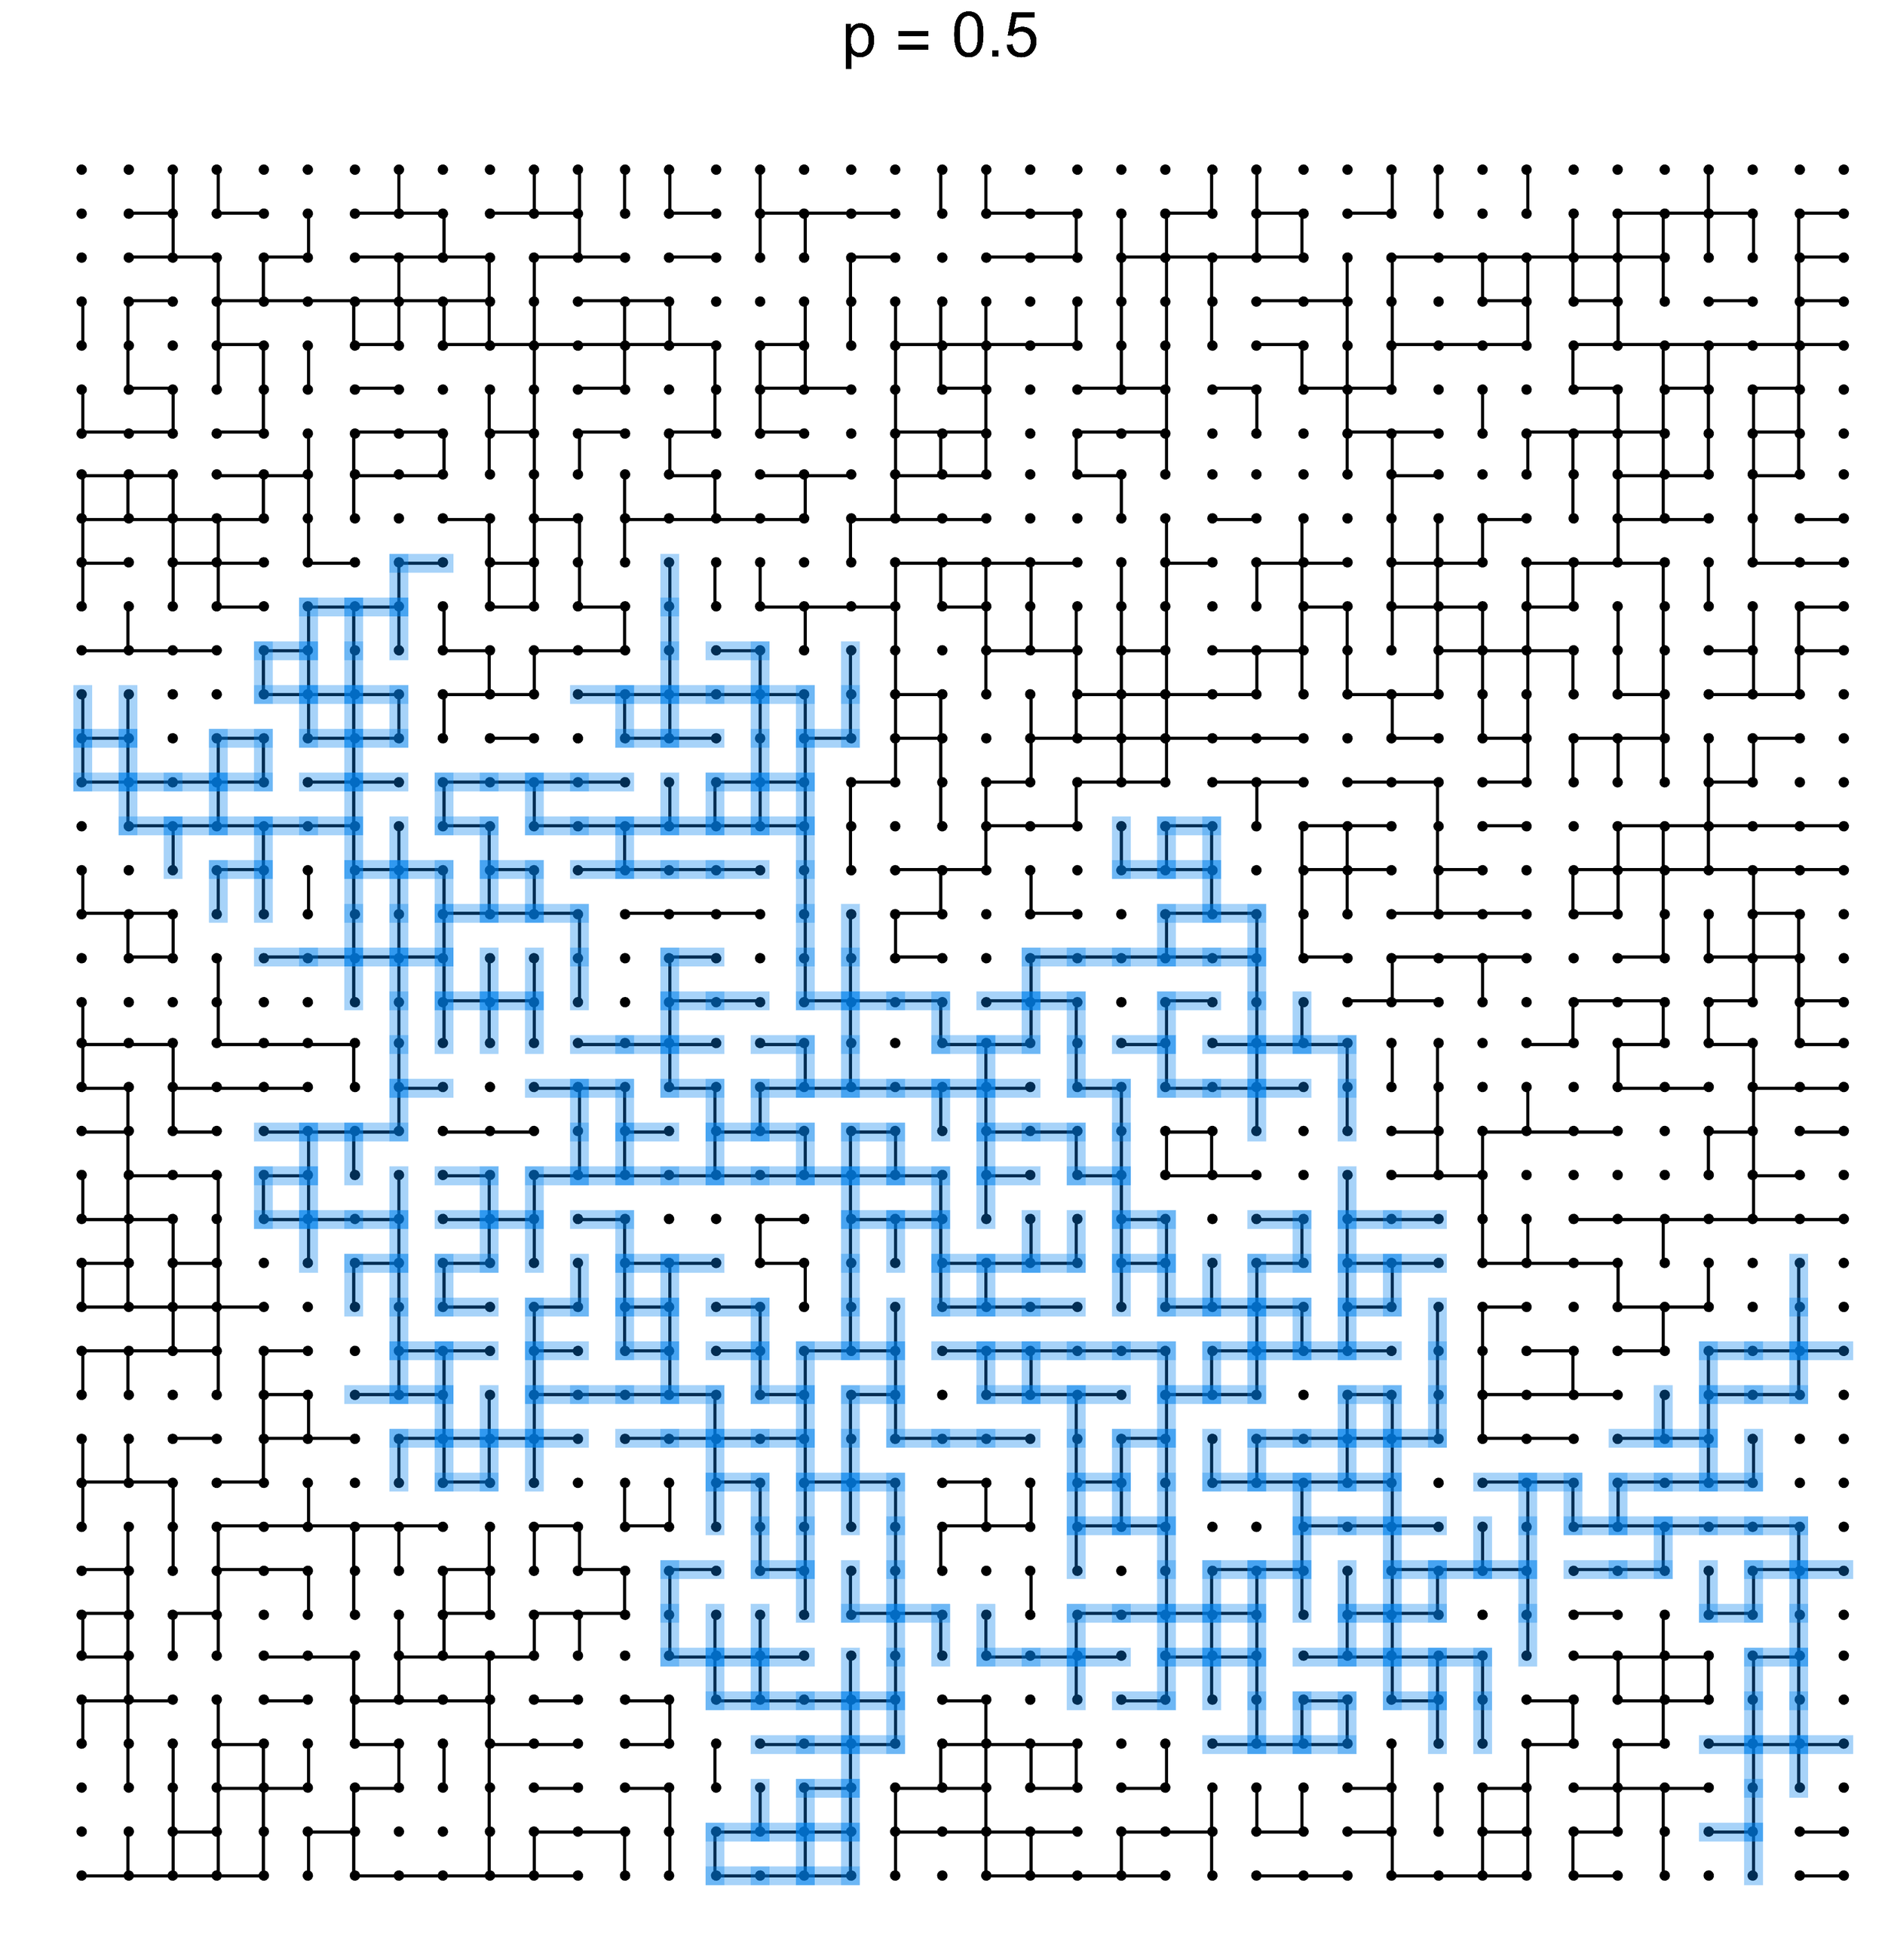
\includegraphics[width=\linewidth]{percolation.png}
    \end{column}
  \end{columns}
\end{frame}

% % Slide 6: Symmetry Classes \& Bipartite Lattice
% \begin{frame}{Symmetry Classes \& Bipartite Lattice}
%   \begin{itemize}
%     \item \textbf{Chiral Symmetry}:
%       \begin{itemize}
%         \item Simple Cubic (SC) lattice is bipartite (A and B sublattices).
%         \item Band center $E=0$: Chiral Orthogonal (BDI) class.
%         \item Result: Anomalously strong localization ($p_q \to 1$).
%       \end{itemize}
%     \vspace{0.4cm}
%     \item \textbf{Orthogonal Symmetry Class (AI)}:
%       \begin{itemize}
%         \item Shift energy to $E = 3.1t$.
%         \item Breaks chiral symmetry, avoids band-center crossover.
%         \item Standard Orthogonal class AI (universal transition).
%         \item Critical exponent expected: $\nu \approx 1.62$.
%       \end{itemize}
%   \end{itemize}
% \end{frame}

\section{Methodology}

% Slide 7: Transfer Matrix Method (TMM)
\begin{frame}{Transfer Matrix Method (TMM)}
  \begin{columns}
    \begin{column}{0.5\textwidth}
      \textbf{Recurrence \& Transfer Matrix}:
      \begin{itemize}
        \item Bar domain $M \times M \times L$ with $L \gg M$.
        \item Solve statics. Time independent Schrodinger
        \item Recurrence on coupled slices (second-order):
          $$C_{l, l-1} \psi_{l-1} + H_l \psi_l + C_{l, l+1} \psi_{l+1} = E \psi_l$$
        \item First-order recurrence product:
          $$\begin{pmatrix} \psi_{l+1} \\ \psi_l \end{pmatrix} = T_l \begin{pmatrix} \psi_l \\ \psi_{l-1} \end{pmatrix}$$
        \item For SC lattice ($C_{l,l\pm1} = -t\mathbf{I}$):
          $$T_l = \begin{pmatrix} \frac{H_l - E\mathbf{I}}{t} & -\mathbf{I} \\ \mathbf{I} & \mathbf{0} \end{pmatrix}$$
      \end{itemize}
    \end{column}
    \begin{column}{0.5\textwidth}
      \textbf{Lyapunov Exponents \& Localization}:
      \begin{itemize}
        \item Global transmission: $\mathcal{M}_L = \prod_{l=1}^L T_l$.
        \item Limiting matrix (Oseledec theorem):
          $$\Gamma = \lim_{L \to \infty} \left( \mathcal{M}_L^\dagger \mathcal{M}_L \right)^{\frac{1}{2L}}$$
        \item Exponents occur in conjugate pairs $\pm\gamma_i$.
        \item Localization length: $\xi_M = 1/\langle \gamma_{\text{min}} \rangle$
        \item Dimensionless localization length
          $$\Lambda_M = \frac{\xi_M}{M}$$
        \item Self-averaging: average $\gamma_i$, \textbf{not} $\xi_M$.
      \end{itemize}
    \end{column}
  \end{columns}
\end{frame}

% % Slide 8: Slice Propagation Algorithm
% \begin{frame}{Slice Propagation Algorithm}
%   \textbf{Objective}: Prevent numerical exponential overflow and preserve channel independence.
%   \begin{block}{Transfer Matrix Method with Reorthogonalization}
%     \begin{enumerate}
%       \item \textbf{Initialize}: State $Q = \mathbf{I}_{2M^2 \times 2M^2}$, accumulator $S = \mathbf{0}_{M^2}$.
%       \item \textbf{Propagate} ($l = 1 \dots L$):
%         \begin{itemize}
%           \item Draw $\epsilon_i$ for slice $l$, build $H_l$, construct transfer matrix $T_l$.
%           \item Update state: $Q \leftarrow T_l Q$.
%         \end{itemize}
%       \item \textbf{Reorthogonalize} (interval $I_{\text{orth}}$):
%         \begin{itemize}
%           \item Modified Gram-Schmidt QR decomposition: $Q = Q' R$.
%           \item Accumulate: $S_i \leftarrow S_i + \ln |R_{ii}|$ for $i=1 \dots M^2$.
%           \item Reset state matrix: $Q \leftarrow Q'$.
%         \end{itemize}
%       \item \textbf{Final Exponents}: $\gamma_i = S_i / L$ for $i=1 \dots M^2$.
%     \end{enumerate}
%   \end{block}
% \end{frame}

% Slide 9: Finite-Size Scaling (FSS) Hypothesis
\begin{frame}{Finite-Size Scaling (FSS) Hypothesis}
  \begin{itemize}
    \item \textbf{Basic Scaling Function}:
      \begin{equation}
      \Lambda_M(x, M) = F\left( \frac{M}{\xi(x)} \right) = F\left( M^{1/\nu} \chi_r(x) \right)
      \end{equation}
      \begin{itemize}
        \item $\chi_r(x) \approx c_r (x - x_c)$ is relevant scaling variable.
        \item $\nu$: Critical exponent.
      \end{itemize}
    \vspace{0.1cm}
    \item \textbf{Irrelevant Scaling Corrections} (for small $M$):
      \begin{equation}
      \Lambda_M(x, M) = F\left( \chi_r(x) M^{1/\nu}, \chi_i(x) M^{-y} \right)
      \end{equation}
      \begin{itemize}
        \item $\chi_i(x)$: Irrelevant scaling variable.
        \item $y > 0$: Irrelevant exponent governing correction decay.
      \end{itemize}
    \vspace{0.1cm}
    \item \textbf{Slevin-Ohtsuki Polynomial Expansion}:
      \begin{equation}
      \Lambda_M(x, M) = \sum_{j=0}^{n_r} \chi_r(x)^j M^{j/\nu} \left( \sum_{k=0}^{n_i} \chi_i(x)^k M^{-k y} a_{j,k} \right)
      \end{equation}
  \end{itemize}
\end{frame}

\section{Numerical Results}

% Slide 10: Results: Anderson Crossing
\begin{frame}{Results: Anderson Crossing}
  \begin{columns}
    \begin{column}{0.5\textwidth}
      \textbf{Configuration}:
      \begin{itemize}
        \item $E=0, p=1$.
        \item Sizes $M \in \{4, 6, 8, 10\}$.
        \item Fit window $W \in [15.0, 18.5]$, $n_r = 4$.
        \item Fixed irrelevant exponent $y = 1.12$.
      \end{itemize}
      \vspace{0.3cm}
      \textbf{Critical Potential} $W_c$:
      \begin{itemize}
        \item \textbf{Obtained}: $16.6174 \pm 0.0156 \text{ (stat)} \pm 0.0148 \text{ (syst)}$
        \item \textbf{Lit}: $16.54$ (Slevin \& Ohtsuki 1999)
      \end{itemize}
      \vspace{0.3cm}
      \textbf{Goodness of Fit}:
      \begin{itemize}
        \item $\chi^2/\text{dof} = 2.421$ (ideally should be close to 1)
      \end{itemize}
    \end{column}
    \begin{column}{0.5\textwidth}
      \centering
      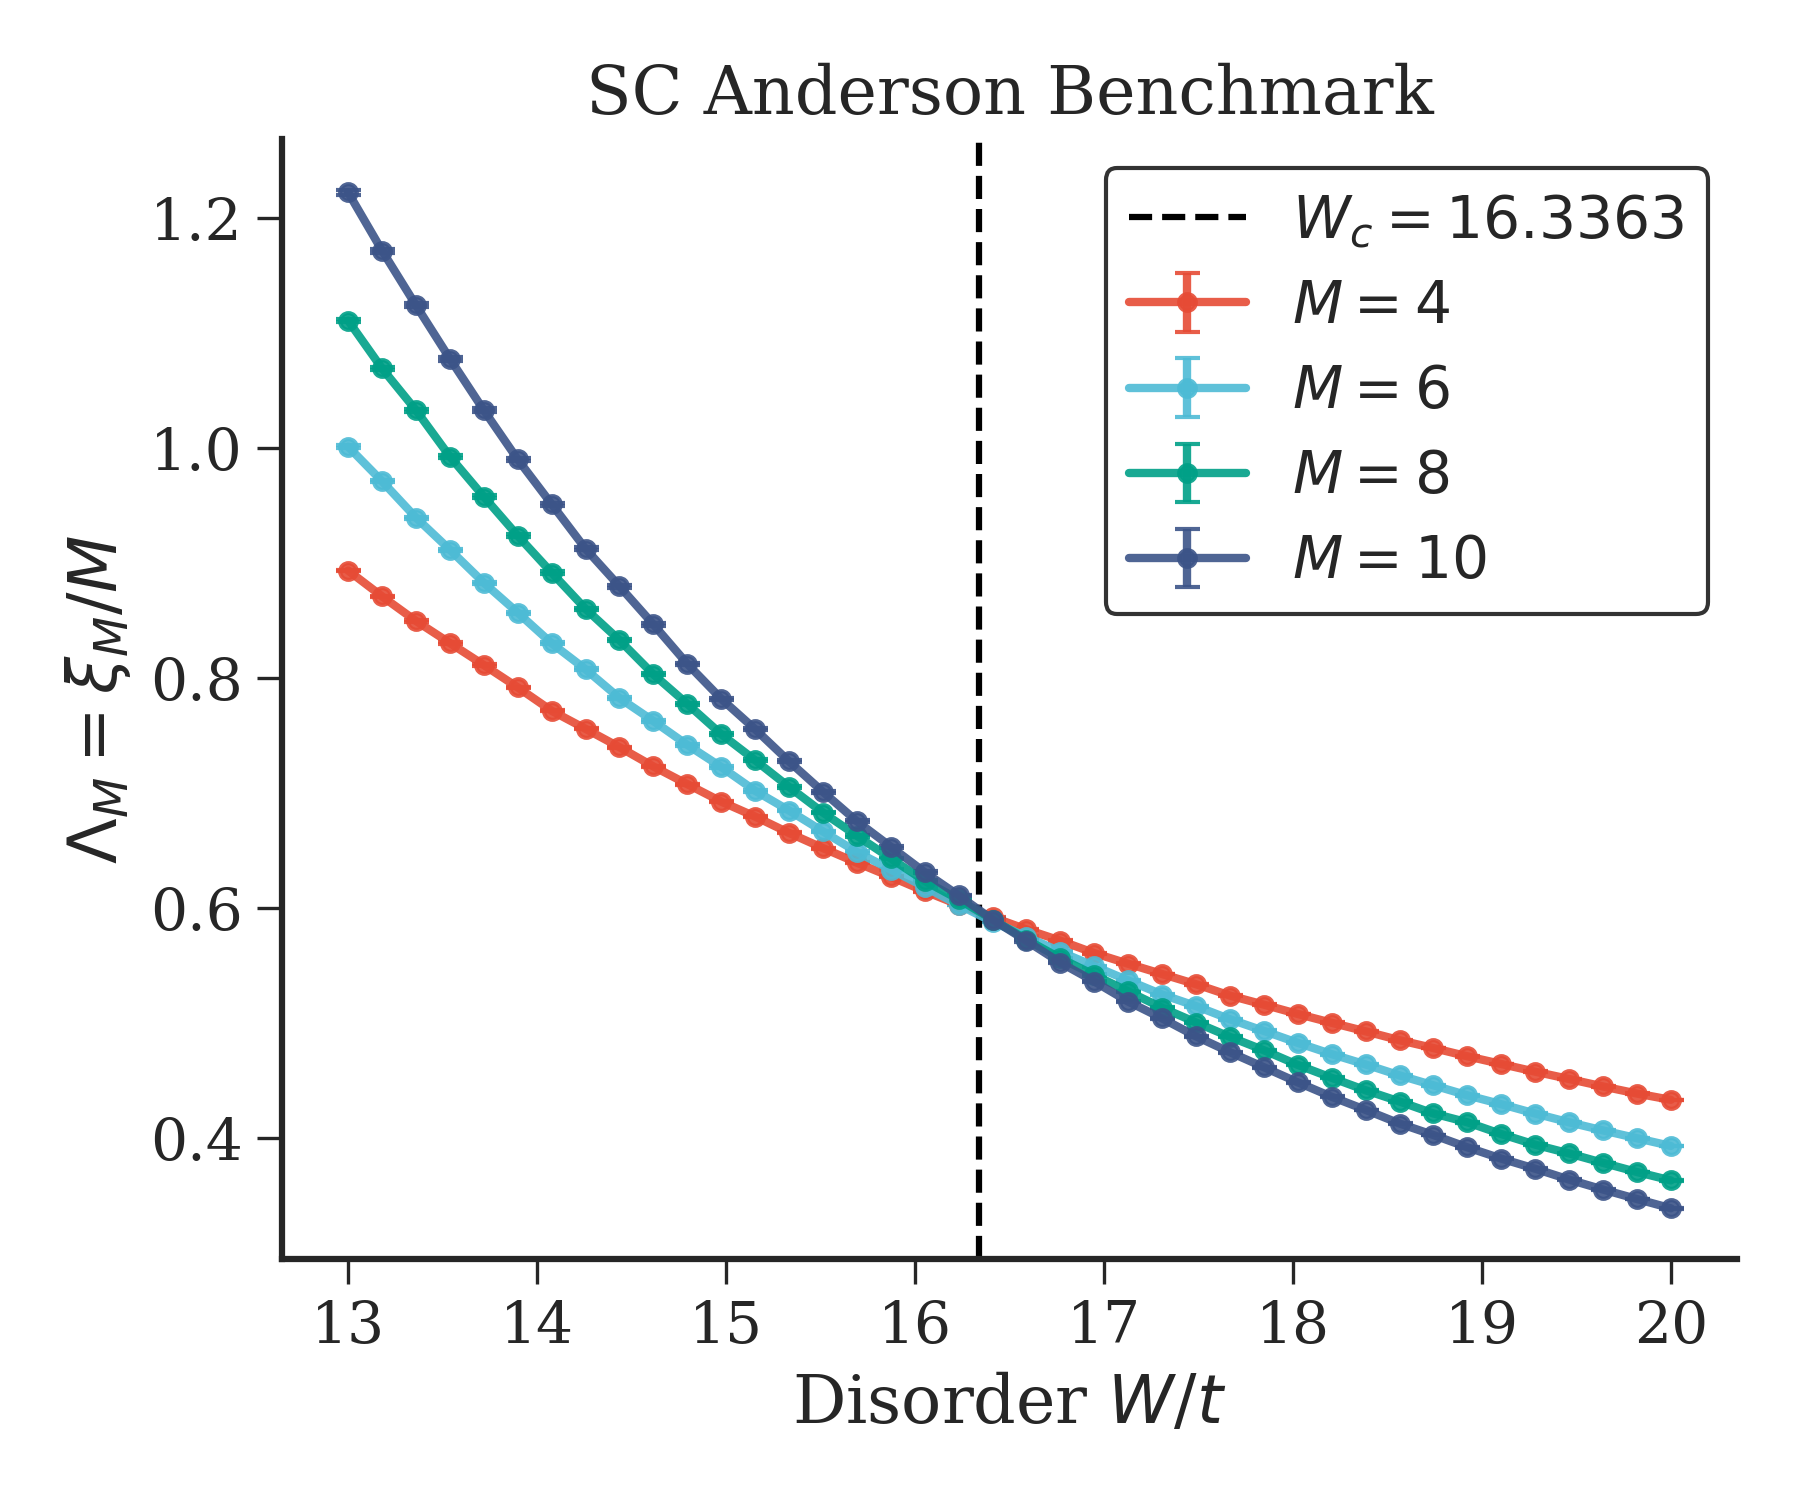
\includegraphics[width=\linewidth]{pub_sc_bench_crossing.png}
    \end{column}
  \end{columns}
\end{frame}

% Slide 11: Results: Anderson Collapse
\begin{frame}{Results: Anderson Collapse}
  \begin{columns}
    \begin{column}{0.5\textwidth}
      \textbf{Configuration}:
      \begin{itemize}
        \item $E=0, p=1$.
        \item Sizes $M \in \{4, 6, 8, 10\}$.
        \item Fit window $W \in [15.0, 18.5]$, $n_r = 4$.
        \item Fixed irrelevant exponent $y = 1.12$.
      \end{itemize}
      \vspace{0.3cm}
      \textbf{Critical Exponent} $\nu$:
      \begin{itemize}
        \item \textbf{Obtained}: $1.6205 \pm 0.0085 \text{ (stat)} \pm 0.0052 \text{ (syst)}$
        \item \textbf{Lit}: $1.571 \pm 0.007$
      \end{itemize}
      \vspace{0.3cm}
      \textbf{Correction Amplitude} $b$:
      \begin{itemize}
        \item $b = 0.0958 \pm 0.0045 \text{ (stat)}$
      \end{itemize}
    \end{column}
    \begin{column}{0.5\textwidth}
      \centering
      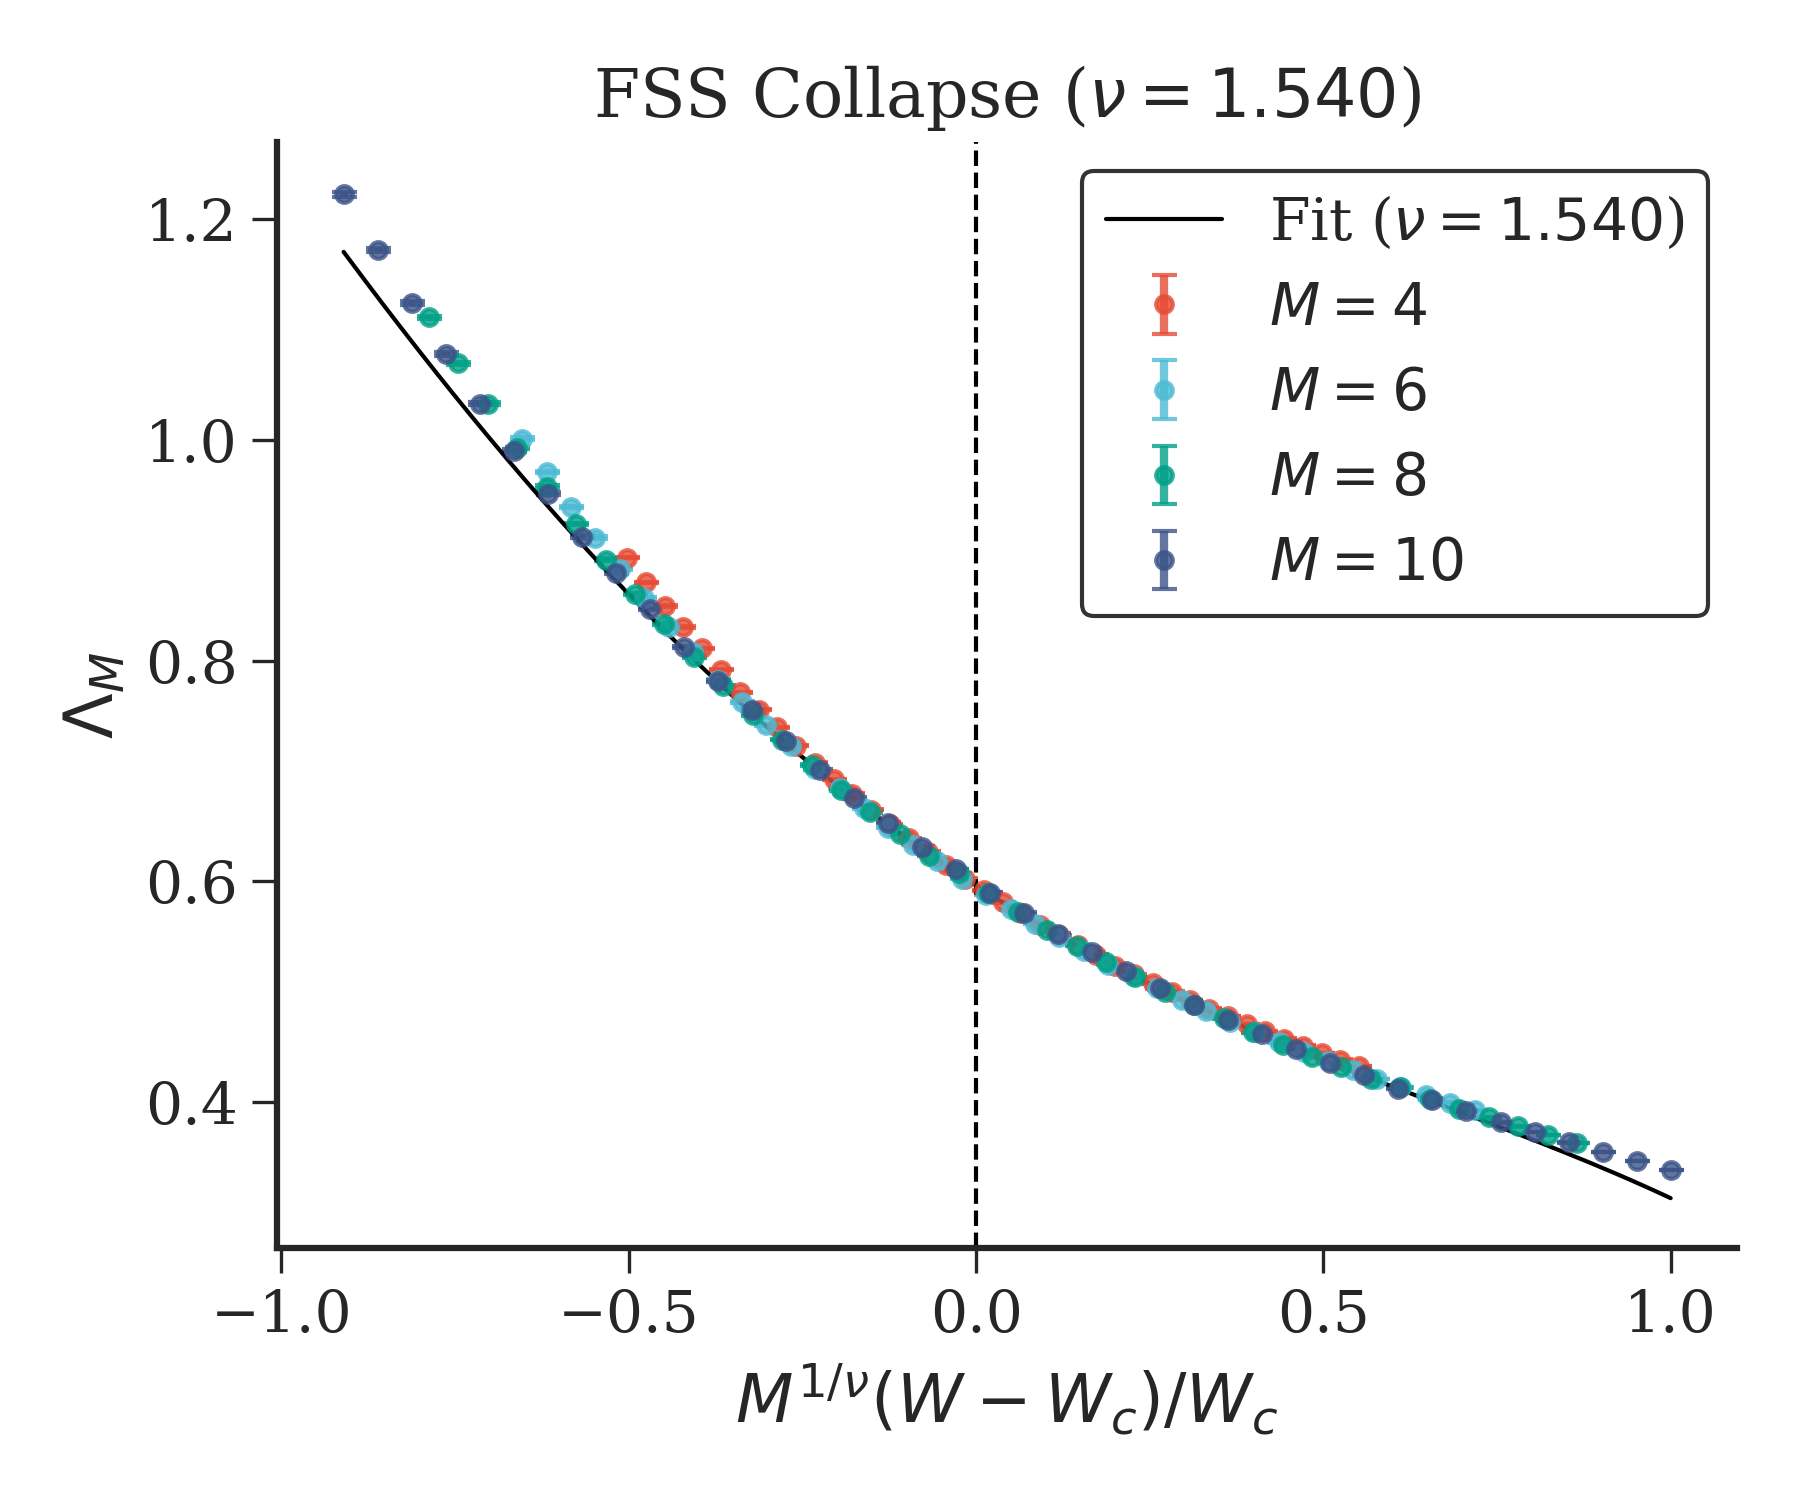
\includegraphics[width=\linewidth]{pub_sc_bench_collapse.png}
    \end{column}
  \end{columns}
\end{frame}

% Slide 12: Classical Percolation Crossover
\begin{frame}{Classical Percolation Crossover}
  \begin{itemize}
    \item \textbf{Tension}: Classical correlation length $\xi_{\text{perc}}$ vs system width $M$.
    \item \textbf{Correlation Length near Window Edge} ($p \approx 0.48$):
      \begin{equation}
      \xi_{\text{perc}} \approx (p - p_c^{\text{cl}})^{-\nu_{\text{perc}}} \approx (0.48 - 0.3115)^{-0.876} \approx 4.6
      \end{equation}
    \item \textbf{Geometric Contamination}:
      \begin{itemize}
        \item $M=4, 6$: Classically constrained ($M \le \xi_{\text{perc}}$) (we cannot use these).
        \item $M=8$: Severely contaminated ($M/\xi_{\text{perc}} \approx 1.7$) (we chose to discard it).
          \begin{itemize}
          \item Optimization collapses into unphysical local minimum.
          \item Massive $+0.024$ bias in critical threshold ($p_q = 0.530$).
          \item Artificially large, negative correction: $b \approx -1.92$.
        \end{itemize}
      \end{itemize}
    \item \textbf{Solution}: Use only $M \in \{10, 12\}$ to isolate quantum transition.
  \end{itemize}
\end{frame}

% Slide 13: Results: Quantum Percolation Crossing
\begin{frame}{Results: Quantum Percolation Crossing}
  \begin{columns}
    \begin{column}{0.5\textwidth}
      \textbf{Configuration}:
      \begin{itemize}
        \item $E=3.1t$.
        \item Clean sizes $M \in \{10, 12\}$.
        \item Fit window $p \in [0.46, 0.54]$, $n_r = 4$.
        \item Fixed irrelevant exponent $y = 1.12$.
      \end{itemize}
      \vspace{0.3cm}
      \textbf{Percolation Threshold} $p_q$:
      \begin{itemize}
        \item \textbf{Obtained}: $0.51670 \pm 0.00456 \text{ (stat)} \pm 0.00450 \text{ (syst)}$
        \item \textbf{Lit}: $0.50628$
      \end{itemize}
      \vspace{0.3cm}
      \textbf{Goodness of Fit}:
      \begin{itemize}
        \item $\chi^2/\text{dof} = 1.068$, $Q = 0.362$
        \item Two widths. Crossings are at $0.482$ and $0.502$. This fit sits above both.
      \end{itemize}
    \end{column}
    \begin{column}{0.5\textwidth}
      \centering
      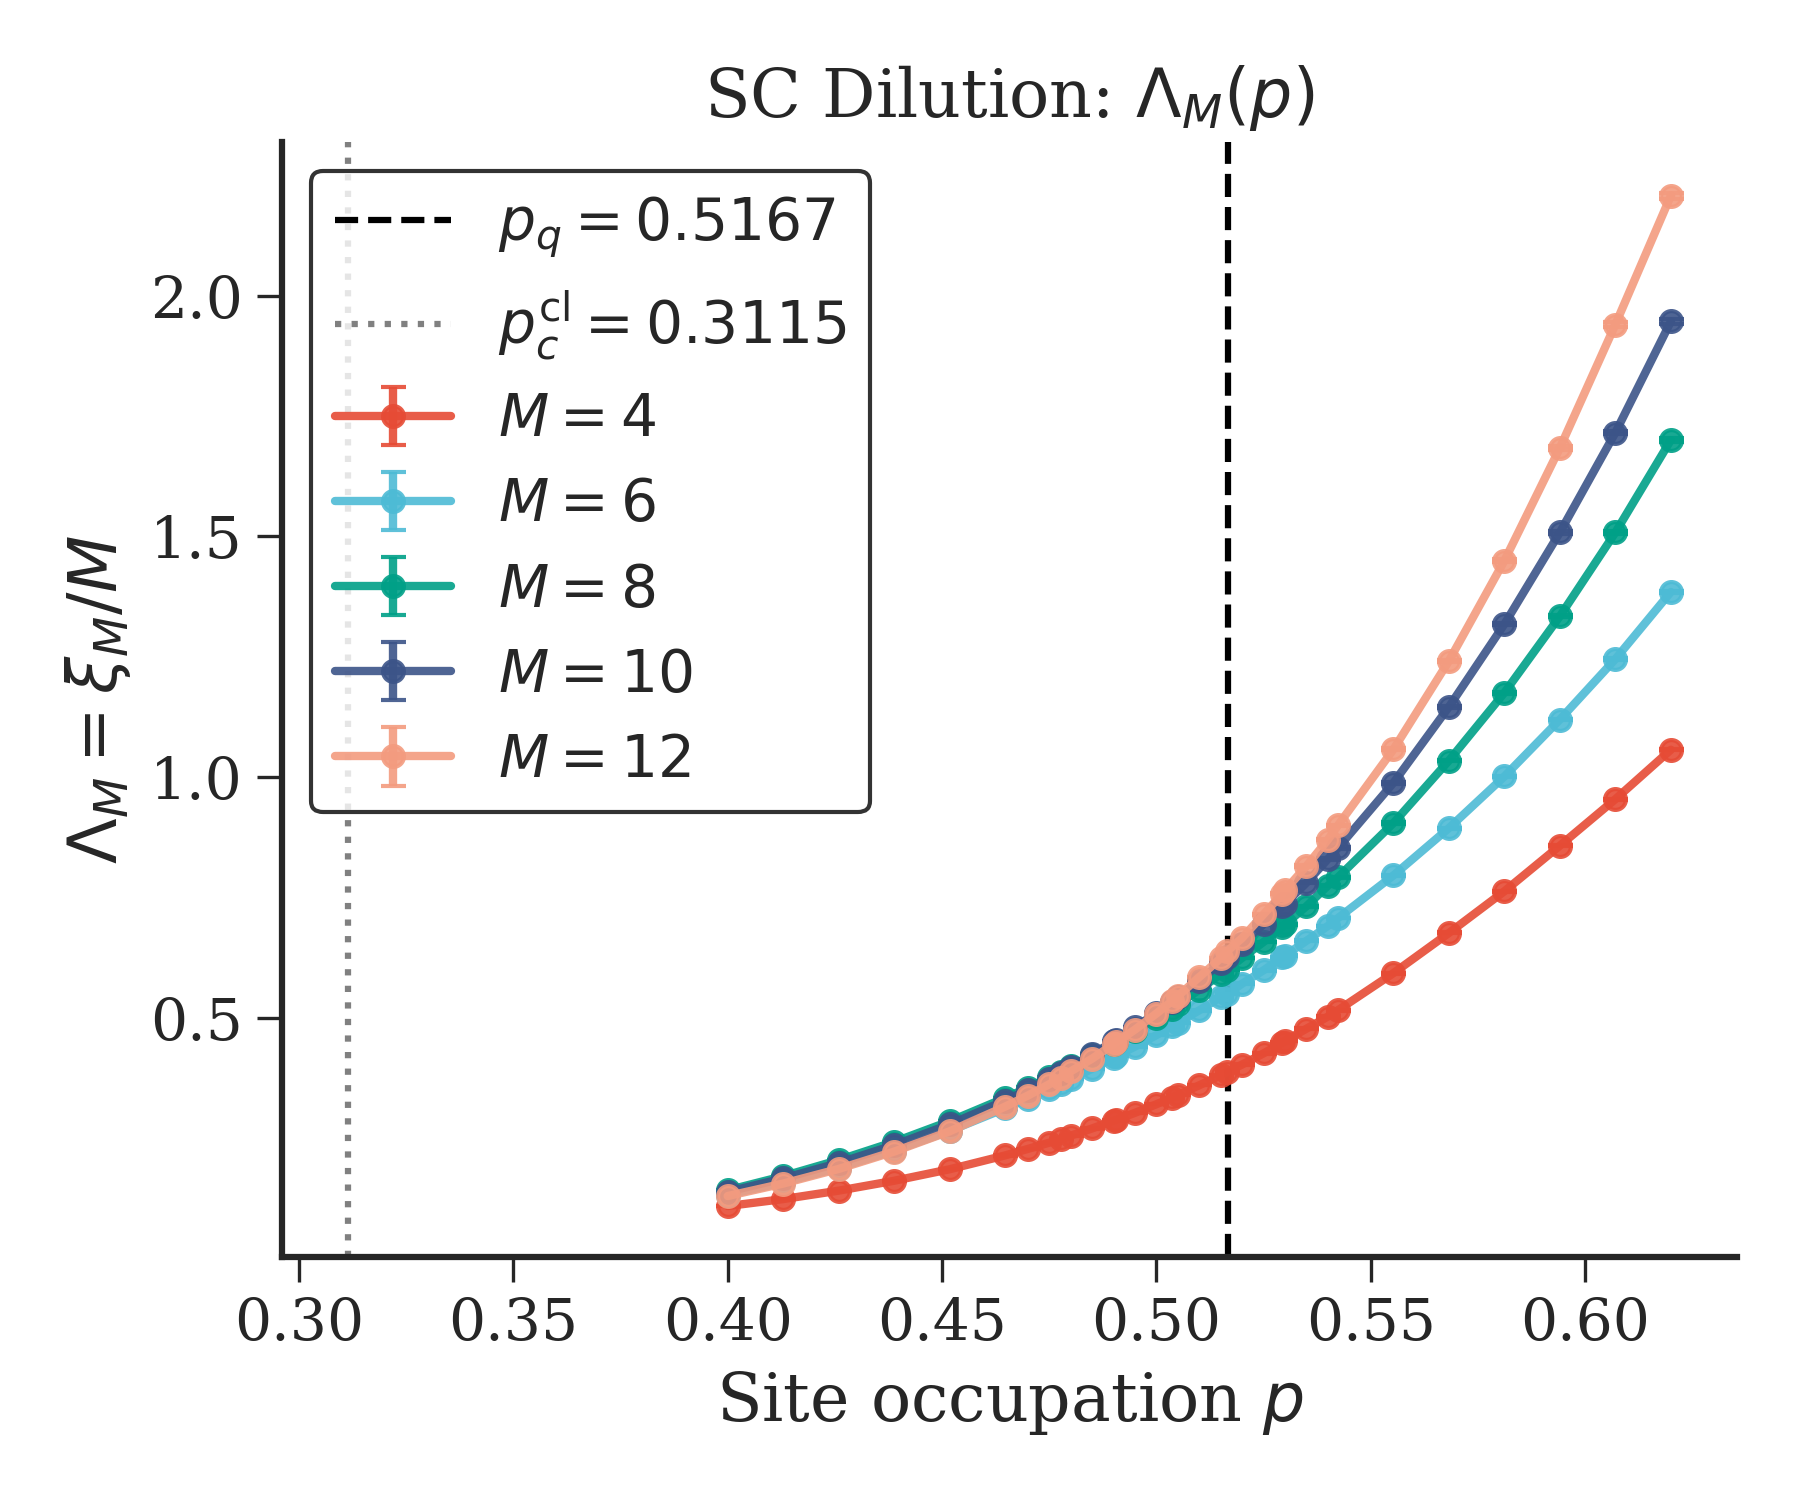
\includegraphics[width=\linewidth]{pub_sc_dilut_crossing.png}
    \end{column}
  \end{columns}
\end{frame}

% Slide 14: Results: Quantum Percolation Collapse
\begin{frame}{Results: Quantum Percolation Collapse}
  \begin{columns}
    \begin{column}{0.5\textwidth}
      \textbf{Configuration}:
      \begin{itemize}
        \item $E=3.1t$.
        \item Clean sizes $M \in \{10, 12\}$.
        \item Fit window $p \in [0.46, 0.54]$, $n_r = 4$.
        \item Fixed irrelevant exponent $y = 1.12$.
      \end{itemize}
      \vspace{0.3cm}
      \textbf{Critical Exponent} $\nu$:
      \begin{itemize}
        \item \textbf{Obtained}: $1.5992 \pm 0.1107 \text{ (stat)} \pm 0.1119 \text{ (syst)}$
        \item \textbf{Lit}: $1.622$ (Orthogonal AI)
        \item Consistent within error.
      \end{itemize}
      \vspace{0.3cm}
    \end{column}
    \begin{column}{0.5\textwidth}
      \centering
      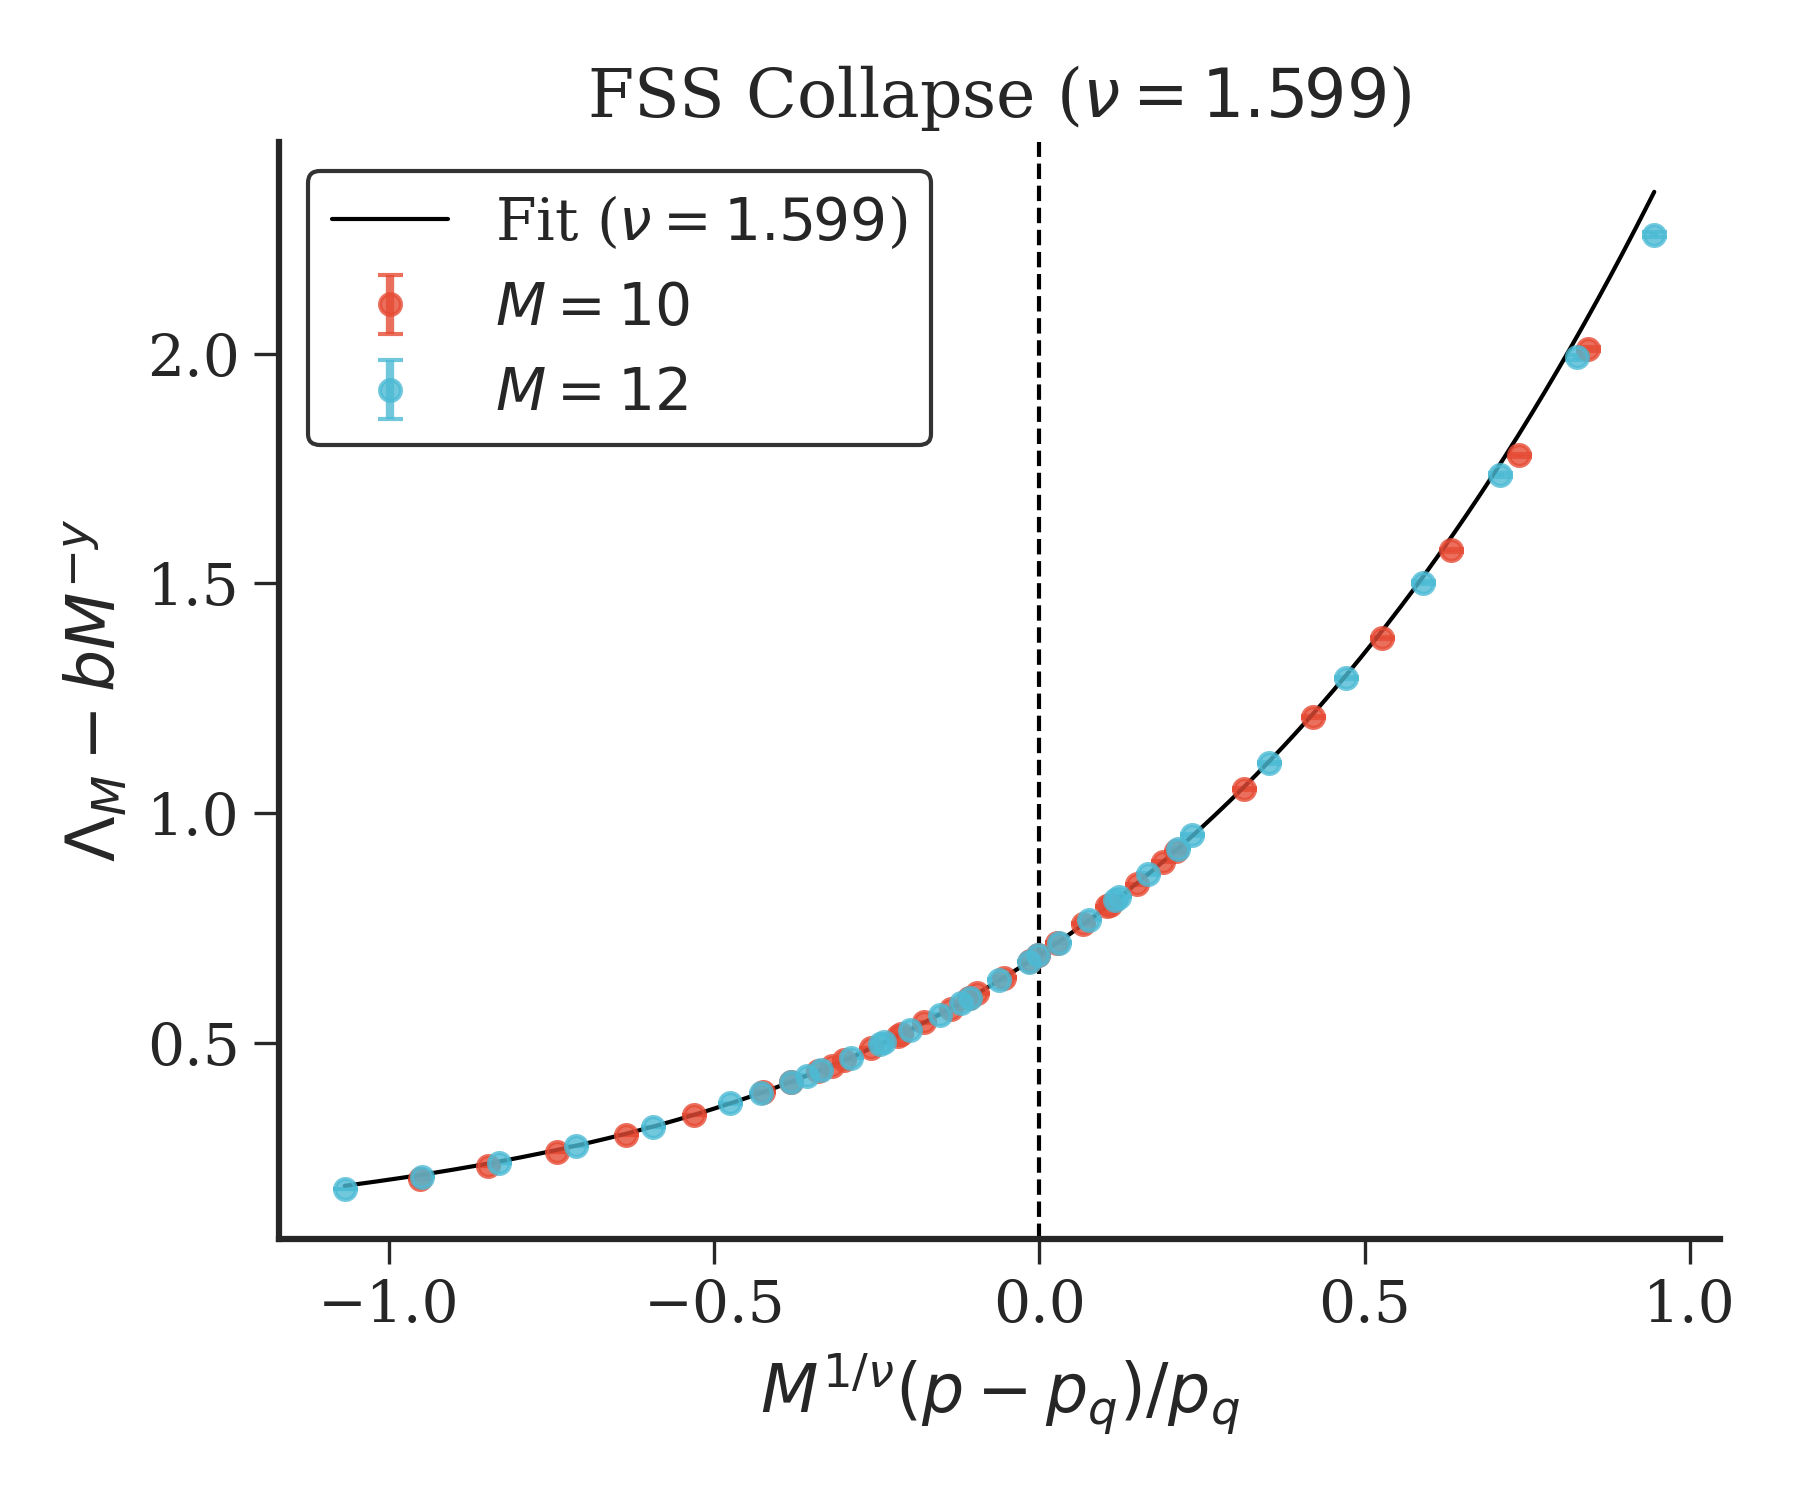
\includegraphics[width=\linewidth]{pub_sc_dilut_collapse.png}
    \end{column}
  \end{columns}
\end{frame}

% Slide 15: Limitations & Challenges
\begin{frame}{Limitations \& Challenges}
  \begin{itemize}
    \item \textbf{Underconstrained Scaling Fit}:
      \begin{itemize}
        \item Only two system sizes ($M=10, 12$) usable for dilution.
        \item Irrelevant exponent $y$ cannot be freely fitted (fixed to $y=1.12$).
      \end{itemize}
    \vspace{0.3cm}
    \item \textbf{Optimizer Instabilities}:
      \begin{itemize}
        \item Highly sensitive to initial parameters.
        \item Trapped in unphysical local minima without initial guess $p_q \approx 0.502$.
      \end{itemize}
    \vspace{0.3cm}
    \item \textbf{Future Directions}:
      \begin{itemize}
        \item Compute larger system widths ($M \ge 14$).
        \item Perform unconstrained scaling analysis with free $y$.
      \end{itemize}
  \end{itemize}
\end{frame}

% Slide 16: Next steps: BCC and FCC
\begin{frame}{Next steps: BCC and FCC}
  \begin{columns}[T]
    \begin{column}{0.48\textwidth}
      \textbf{Body-Centered Cubic (BCC)}
      \begin{itemize}
        \item \textbf{Coordination:} $Z=6 \rightarrow 8$.
        \item \textbf{Threshold:} $p_c$ drops to $\approx 0.246$.
        \item \textbf{Symmetry:} Bipartite. Requires evaluating at $E=3.1t$ to access Orthogonal AI class.
        \item \textbf{Cost:} 2-atom basis ($2M^2$ vector). $\mathcal{O}(N^3)$ scaling incurs an \textbf{$8\times$ penalty}.
      \end{itemize}
    \end{column}
    
    \begin{column}{0.48\textwidth}
      \textbf{Face-Centered Cubic (FCC)}
      \begin{itemize}
        \item \textbf{Coordination:} Maximum $Z=12$.
        \item \textbf{Threshold:} $p_c$ plummets to $\approx 0.199$.
        \item \textbf{Symmetry:} Not bipartite (triangles). Natively Orthogonal AI (Altland-Zirnbauer) at exact band center ($E=0$).
        \item \textbf{Cost:} 4-atom basis ($4M^2$ vector). $\mathcal{O}(N^3)$ scaling incurs a \textbf{$64\times$ penalty}.
      \end{itemize}
    \end{column}
  \end{columns}
\end{frame}

% Slide 17: Conclusions
\begin{frame}{Conclusions}
  \begin{itemize}
    \item We developed a JAX-accelerated implementation of the Transfer Matrix Method.
    \item We validated the TMM solver against the 3D Anderson localization transition.
    \item We identified classical percolation crossover effects that contaminate small system sizes.
    \item We isolated the quantum percolation threshold by restricting the scaling fit to $M \ge 10$.
    \item We extracted a critical exponent consistent with the 3D Orthogonal universality class.
  \end{itemize}
\end{frame}

\end{document}
